\begin{center}
\Huge
Binomialkoefficienten
\end{center}

\section*{Binomialkoefficienten}
\stepcounter{section}
Vi diskuterede sidste gang permutationer og antallet af permutationer af $r$ elementer blandt $n$ elementer. I den bearbejdning tog vi ikke højde for, at permutationers rækkefølge ofte er ligegyldig. Trækker vi fem kort i et kortspil, så er vi ligeglade med, om vi har trukket spar to før klør fem eller omvendt. Dette vil vi tage højde for nu. 

\begin{defn}
Vi betegner antallet af måder, vi kan udvælge $r$ elementer blandt $n$ elementer, hvor rækkefølgen ikke har betydning som
\begin{align*}
	\textnormal{K}(n,r) = \binom{n}{r}.
\end{align*}
hvoraf det er den sidste skrivemåde, der er klart mest anvendt uden for gymnasieskolen, men $\textnormal{K}(n,r)$ vil I se i en eksamensopgave. Dette symbol kaldes for binomialkoefficienten.
\end{defn}
\begin{setn}
Binomialkoefficienten $\textnormal{K}(n,r)$ er givet ved
\begin{align*}
	\textnormal{K}(n,r) = \frac{n!}{r!(n-r)!}.
\end{align*}
\end{setn}
\begin{proof}
Antallet af måder, vi kan udvælge $r$ elementer blandt $n$ elementer, hvor rækkefølge har betydning så vi sidst var $\textnormal{P}(n,r) = n!/(n-r)!$. Vi skal nu tage højde for alle de permutationer, der består af de samme elementer i forskellige rækkefølge. Men for ethvert valg af $r$ elementer, så er der jo lige præcis $r!$ måder at permutere dem. Derfor må vi have $r!$ gange for mange permutationer med. Altså er $K(n,r)$ givet ved
\begin{align*}
	\textnormal{K}(n,r) = \frac{\textnormal{P}(n,r)}{r!} = \frac{\frac{n!}{(n-r)!}}{r!} = \frac{n!}{r!(n-r)!}.
\end{align*}
\end{proof}

\begin{exa}
	Hvis der for en mængde $A$ gælder, at $|A| = n$, så er $\textnormal{K}(n,r)$ antallet af delmængder af $A$ med kardinalitet $r$, da rækkefølgen af elementerne ikke har
	betydning i en mængde.
\end{exa}
\begin{exa}
	Vi skal bestemme på hvor mange måder, vi kan udvælge 3 kort i et kortspil. Da rækkefølge ikke betyder noget, og da der er 52 kort i et kortspil, så er det givet som
	\begin{align*}
		\binom{52}{3} = \frac{52!}{3!(49)!} = 21000.
	\end{align*}
\end{exa}

\subsection*{Pascals trekant}

Pascals trekant er defineret som en uendelig trekant af binomialkoefficienter. De første seks rækker kan ses af Figur \ref{fig:pascal}.
\begin{figure}[H]
	\centering
	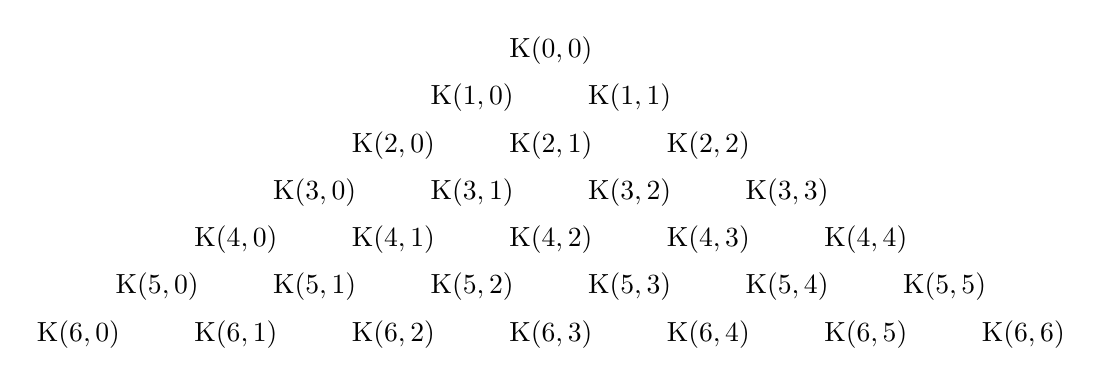
\begin{tikzpicture}
		\node at (0,0) {K$(0,0)$};
		\node at (-1,-0.6) {K$(1,0)$};
		\node at (1, -0.6) {K$(1,1)$};
		\node at (-2,-1.2) {K$(2,0)$};
		\node at (0,-1.2) {K$(2,1)$};
		\node at (2,-1.2) {K$(2,2)$};
		\node at (-3,-1.8) {K$(3,0)$};
		\node at (-1,-1.8) {K$(3,1)$};
		\node at (1,-1.8) {K$(3,2)$};
		\node at (3,-1.8) {K$(3,3)$};
		\node at (-4,-2.4) {K$(4,0)$};
		\node at (-2,-2.4) {K$(4,1)$};
		\node at (0,-2.4) {K$(4,2)$};
		\node at (2,-2.4) {K$(4,3)$};
		\node at (4,-2.4) {K$(4,4)$};
		\node at (-5,-3.0) {K$(5,0)$};
		\node at (-3,-3.0) {K$(5,1)$};
		\node at (-1,-3.0) {K$(5,2)$};
		\node at (1,-3.0) {K$(5,3)$};
		\node at (3,-3.0) {K$(5,4)$};
		\node at (5,-3.0) {K$(5,5)$};
		\node at (-6,-3.6) {K$(6,0)$};
		\node at (-4,-3.6) {K$(6,1)$};
		\node at (-2,-3.6) {K$(6,2)$};
		\node at (-0,-3.6) {K$(6,3)$};
		\node at (2,-3.6) {K$(6,4)$};
		\node at (4,-3.6) {K$(6,5)$};
		\node at (6,-3.6) {K$(6,6)$};
	\end{tikzpicture}
	\caption{De første seks rækker i Pascals trekant}
	\label{fig:pascal}
\end{figure}
Det er klart, at alle $\textnormal{K}(n,0) = 1$ og $\textnormal{K}(n,n) = 1$ for alle $n\in \mathbb{N}$. Dette sammen med rekursionsligningen \eqref{eq:rekursion} kan hjælpe os med at udfylde Pascals trekant. Resultatet af dette kan ses af Figur \ref{fig:pascal2}.
\begin{figure}[H]
	\centering
	\begin{tikzpicture}
		\node at (0,0) {1};
		\node at (-1,-0.6) {1};
		\node at (1, -0.6) {1};
		\node at (-2,-1.2) {1};
		\node at (0,-1.2) {2};
		\node at (2,-1.2) {1};
		\node at (-3,-1.8) {1};
		\node at (-1,-1.8) {3};
		\node at (1,-1.8) {3};
		\node at (3,-1.8) {1};
		\node at (-4,-2.4) {1};
		\node at (-2,-2.4) {4};
		\node at (0,-2.4) {6};
		\node at (2,-2.4) {4};
		\node at (4,-2.4) {1};
		\node at (-5,-3.0) {1};
		\node at (-3,-3.0) {5};
		\node at (-1,-3.0) {10};
		\node at (1,-3.0) {10};
		\node at (3,-3.0) {5};
		\node at (5,-3.0) {1};
		\node at (-6,-3.6) {1};
		\node at (-4,-3.6) {6};
		\node at (-2,-3.6) {15};
		\node at (-0,-3.6) {20};
		\node at (2,-3.6) {15};
		\node at (4,-3.6) {6};
		\node at (6,-3.6) {1};
	\end{tikzpicture}
	\caption{De første seks rækker i Pascals trekant.}
	\label{fig:pascal2}
\end{figure}
\subsection*{Opgave 1}
Vi har en pose med fem forskellige bolde. 
\begin{enumerate}[label=\roman*)]
	\item På hvor mange forskellige måder kan vi vælge to bolde i posen, hvis rækkefølgen ikke betyder noget?
	\item På hvor mange forskellige måder kan vi vælge 4 bolde i posen, hvis rækkefølgen ikke betyder noget?
\end{enumerate}

\subsection*{Opgave 2}
En isbutik har 12 forskellige typer is, og vi er ligeglade med rækkefølgen af kugler
\begin{enumerate}[label=\roman*)]
	\item På hvor mange forskellige måder kan vi bestille 3 kugler is?
	\item Hvis vi vil have chokolade som den sidste kugle, på hvor mange forskellige måder kan vi så bestille is?
	\item Hvis vi vil have chokolade, men er ligeglade med placeringen, på hvor mange forskellige måder kan vi så
	 bestille en is?
\end{enumerate}

\subsection*{Opgave 3}
\begin{enumerate}[label=\roman*)]
	\item Opskriv den 7. række i Pascals trekant
	\item Af Pascals trekant ser det ud som om, at 
	\begin{align*}
		\textnormal{K}(n,r) = \textnormal{K}(n,n-r).
	\end{align*}
	Giv et kombinatorisk argument for, hvorfor dette er sandt. (Forklar det uden at regne)
\end{enumerate}

\subsection*{Opgave 4}
Bestem ved hjælp af Pascals trekant følgende binomialkoefficienter:
\begin{align*}
	&1) \ \textnormal{K}(3,4)  &&2) \ \textnormal{K}(7,3) \\
	&3) \ \textnormal{K}(8,5)  &&4) \ \binom{9}{2} \\
\end{align*}


\subsection*{Opgave 5}
I skal lave netværksgrupper i klassen. Disse består af 4 personer.
\begin{enumerate}[label=\roman*)]
	\item Bestem antallet af måder, man kan lave en netværksgruppe. 
\end{enumerate}


\subsection*{Opgave 6}
En mand har i sit klædeskab syv skjorter, fem par bukser og 3 jakker. Han skal have tre skjorter, to par bukser og en jakke med på ferie. På hvor mange måder kan han pakke sin kuffert?

\subsection*{Opgave 7}
Vi er til dimission og alle får serveret et glas champagne. Alle gæster skåler med alle andre gæster, og vi hører i alt 435 klir fra glas, der støder sammen.
\begin{enumerate}[label=\roman*)]
	\item Hvor mange er der til dimissionen?
	\item Gæsterne skåler nu tre og tre på alle mulige måder. Hvor mange klir hører vi nu?
\end{enumerate}


\subsection*{Opgave 8}
Bestem følgende binomialkoefficienter:
\begin{align*}
&1) \ \binom{7}{2}  &&2) \ \binom{10}{3}  \\
&3) \ \binom{5}{4}  &&4) \ \binom{200}{1}   \\
\end{align*}

\subsection*{Opgave 9}
En pokerhånd består af fem kort fra et kortspil på 52 kort.
\begin{enumerate}[label=\roman*)]
\item Hvor mange hænder er der i poker?
\item En flush består af fem kort i samme kulør. På hvor mange forskellige måder kan man få flush med hjerter? På hvor mange måder kan man få flush i alt?
\item En straight består af 5 kort i følge; e.g. 2,3,4,5,6. På hvor mange forskellige måder kan man få straight?
\end{enumerate} 

\subsection*{Opgave 10}
Du skal i biografen med klassen. I en biograf med 200 sæder, på hvor mange forskellige måder kan I så vælge jeres sæder?

\subsection*{Opgave 11}
Bestem i Maple $(x + y)^n$ for $n = 1,2,\hdots, 6$ og sammenlign koefficienterne for leddene med Pascals trekant. Hvad kan du se?

